\documentclass[12pt,a4paper,twoside]{report}
\usepackage{cs}
\usepackage[T1]{fontenc}
\usepackage[utf8]{inputenc}
\usepackage[english]{babel}
\usepackage{times}
\usepackage{graphicx}
\graphicspath{{figures/}}
\usepackage{latexsym}
\usepackage{amsmath,amsbsy}
\usepackage{amssymb}
\usepackage[matrix,arrow]{xy}
\usepackage{ae,aecompl}
\usepackage{amstext}
\usepackage{graphics}
\usepackage{ae,aecompl}
\usepackage{algorithm}
\usepackage{algpseudocode}
\usepackage{listings}
\usepackage{color}

\definecolor{codegreen}{rgb}{0,0.6,0}
\definecolor{codegray}{rgb}{0.5,0.5,0.5}
\definecolor{codepurple}{rgb}{0.58,0,0.82}
\definecolor{backcolour}{rgb}{0.95,0.95,0.92}

\lstdefinestyle{mystyle}{
    backgroundcolor=\color{backcolour},   
    commentstyle=\color{codegreen},
    keywordstyle=\color{magenta},
    numberstyle=\tiny\color{codegray},
    stringstyle=\color{codepurple},
    basicstyle=\ttfamily\footnotesize,
    breakatwhitespace=false,         
    breaklines=true,                 
    captionpos=b,                    
    keepspaces=true,                 
    numbers=left,                    
    numbersep=5pt,                  
    showspaces=false,                
    showstringspaces=false,
    showtabs=false,                  
    tabsize=2
}
\lstset{style=mystyle}
\usepackage{titlesec}
\usepackage{fancyhdr}
\usepackage{hyperref}
%% decomentati linia urmatoare pentru e nu mai evidenția hiper legăturile pentru imprimare pe hârtie
%\hypersetup{hidelinks}
\usepackage{geometry}
\usepackage{lipsum}
\usepackage{enumitem}
\usepackage{pdfpages}

\setlist{noitemsep,nolistsep}

\DeclareFontFamily{TS1}{aer}{}
\DeclareFontShape{TS1}{aer}{m}{n}{<->ssub * cmr/m/n}{}

\diplomathesis
\centerchapter
\singlespace
\newenvironment{definition}[1][Definition.]{\begin{trivlist}
\item[\hskip \labelsep {\bfseries #1}]}{\end{trivlist}}

%%%%%%%%%%%%%%%%%%%%%%%%%%%%%% Change the last element accordingly
\renewcommand{\thesisauthor}{Sebastian Duică}    %% Your first name(s) and family name.
\renewcommand{\thesismonth}{July}     %% The month of the licence session
\renewcommand{\thesisyear}{2026}      %% The year of the
\renewcommand{\thesistitle}{Real-Time Light Dosimetry for Heritage Digital Twins via Texture Space Ray Tracing} % Title of the thesis
\renewcommand{\thesissupervisor}{Assoc. Prof. Victor Ioan Bâcu} %% Supervisor
%%%%%%%%%%%%%%%%%%%%%%%%%%%%%%%%%%%%%
\newcommand{\makeThesisTitle}{\textbf{\thesistitletypesize \thesistitle}}
\newcommand{\makeThesisType}{\thesistypetypesize \thesistype}
\newcommand{\department}{\sffamily\bfseries\small FACULTY OF AUTOMATION AND COMPUTER SCIENCE}
\renewcommand{\thesistype}{LICENSE THESIS}
\newcommand{\uline}[1]{\rule[0pt]{#1}{0.4pt}}
%\renewcommand{\thesisdedication}{Părinților mei}

% Headings pentru folie de capăt

 \geometry{
	a4paper,
	total={159.2mm,246.2mm},
	left=25.4mm,
	top=25.4mm,
}


\begin{document}
%\frontmatter
%%%%%%%%%%% Stil pentru paginile de capăt
\pagestyle{fancy}
\setlength{\voffset}{-10pt}
\setlength\headheight{70.0pt}
%\addtolength{\textheight}{-80.0pt}
\renewcommand{\headrulewidth}{0pt}
\chead{%
	
\includegraphics[width=\textwidth]{figures/AntetUTCNEng.pdf}
}
\cfoot{}
\lfoot{}
\rfoot{}
%\pagestyle{headings}
%%%%% Thesis title page %%%%%%%%%%%%%%%%%%%%%%%%
\begin{center}
	{\department}

	\vspace{4cm}
	\makeThesisTitle %LICENSE THESIS TITLE
	~\\~\\

	\makeThesisType

	~\\\vspace{6.5cm}

	\begin{tabular}{p{.3\linewidth}p{.5\linewidth}}
	               {\hfill Graduate:}             & {\bf \thesisauthor}    \\
	                                                            &                         \\
	               {\parbox[t]{\linewidth}{\hfill Supervisor:}} & {\bf \thesissupervisor} \\
	\end{tabular}

	\vspace{3cm}
	{\bf \thesisyear}
\end{center}
%%%%%%%%%%%%%%%%% end of thesis title page %%%%%%%%%%%%%%%%%%%%%%%%%%%%%%%%%%%%
\newpage
%%%%%%% Proposal page %%%%%%%%%%%%%%%%%%%%%%%%%%%%%%%
\begin{center}
	{\department}
\end{center}
\vspace{0.5cm}

%\begin{small}
\begin{tabular}{p{7cm}p{8cm}}
	%\hspace{-1cm}& VIZAT,\\
	\hspace{-1cm}DEAN,                             & HEAD OF DEPARTAMENT,                \\
	\hspace{-1cm}{\bf Prof. dr. ing. Vlad MUREȘAN} & {\bf Prof. dr. ing. Rodica POTOLEA} \\
\end{tabular}

\vspace{2cm}

\begin{center}
	Graduate: {\bf \thesisauthor}

	\vspace{1cm}

	{\bf \thesistitle}
\end{center}

\vspace{5mm}

\begin{enumerate}
	\item {\bf Project proposal:} Development of ChronoLux, an interactive Digital Twin for real-time light dosimetry using Texture Space Ray Tracing in DirectX 12.
	\item {\bf Project contents:} Introduction, Project Objectives, Bibliographic Research, Analysis and Theoretical Foundation, Detailed Design and Implementation, Testing and Validation, User's Manual, Conclusions, Bibliography.
	\item {\bf Place of documentation:} Technical University of Cluj-Napoca, Computer Science Department
	\item {\bf Consultants:}
	\item {\bf Date of issue of the proposal:} October 1, 2025
	\item {\bf Date of delivery:} July 10, 2026
\end{enumerate}
\vspace{1.2cm}

\hspace{6cm} Graduate: \uline{6cm}

\vspace{0.5cm}
\hspace{6cm} Supervisor: \uline{5cm}
\newpage
%%%%%%%%%%%%%%%%%% End of proposal page
%%%%%%%%% Page with declaration %%%%%%%%%%%%%%%%%%%%%%%%%%%%%%%%%%%%%%%%%%
\begin{center}
	{\department}
\end{center}
\vspace{1cm}
\begin{center}
	{\bf Declarație pe proprie răspundere privind\\
		autenticitatea lucrării de licență}
\end{center}
\vspace{1cm}

\begin{minipage}{\linewidth}
	Subsemnatul(a) \uline{.73\linewidth},
	\uline{.82\linewidth}
	legitimat(ă) cu\\ \uline{4cm} seria \uline{3cm} nr. \uline{6.3cm}
	(conform copiei anexate prezentei declarații, copie semnată și certificată ”conform cu originalul”), autorul lucrării\
	\uline{\linewidth}
	\uline{\linewidth}
	\uline{\linewidth}
	elaborată în vederea susținerii examenului de finalizare a studiilor de licență la Facultatea de Automatică și Calculatoare, Programul de studiu \uline{10cm} din cadrul Universității Tehnice din Cluj-Napoca, sesiunea \uline{4cm} a anului universitar \uline{3cm}, declar pe proprie răspundere, că această lucrare este rezultatul propriei activități intelectuale, pe baza cercetărilor mele și pe baza informațiilor obținute din surse care au fost citate, în textul lucrării și în bibliografie.\\
	Declar, că această lucrare nu conține porțiuni plagiate, iar sursele bibliografice au fost folosite cu respectarea legislației române și a convențiilor internaționale privind drepturile de autor.\\
	Declar, de asemenea, că această lucrare nu a mai fost prezentată în fața unei alte comisii de examen de licență.\\
	În cazul constatării ulterioare a unor declarații false, voi suporta sancțiunile administrative, respectiv, \emph{anularea examenului de licență}.
	Sunt de acord ca, pe tot parcursul vieții, în cazul în care este necesar și se va dori verificarea autenticității lucrării mele să fiu identificat și verificat în baza datelor declarate de mine și conform copiei documentului de identitate menționat mai sus.
\end{minipage}
\vspace{1.5cm}

Data \hspace{8cm} Nume, Prenume

\vspace{0.5cm}

\uline{3cm} \hspace{5cm} \uline{5cm}

\vspace{1cm}
\hspace{9.4cm}Semnătura
\newpage
%%%%%%%%%%%%%%%%%%% end of page with declaration % the first 3 pages
%%%%%%%%%%%%%%%%% Advices page to remove
\thispagestyle{empty}
% \include{guideline}
\newpage
%%%%%%%%%%%%%%%%%% end of advices page
\pagestyle{fancy}
\setlength\headheight{16.0pt}
\renewcommand{\chaptermark}[1]{\markboth{\chaptername~\thechapter.~#1}{}}
\renewcommand{\sectionmark}[1]{\markright{\thesection\ #1}}
\renewcommand{\headrulewidth}{0.4pt}
\lhead{}
\chead{%
    \leftmark\rightmark
}
\chead{}
\cfoot{\thepage}
\lfoot{}
\rfoot{}

%%%%%%%%%%%% Table of contents
\pagenumbering{roman}
\setcounter{page}{1}

\newpage

\tableofcontents

\newpage

%\listoftables
%\listoffigures

\pagenumbering{arabic}
\setcounter{page}{1}


\titleformat{\chapter}[hang]
{\normalfont\Large\bfseries}{\chaptertitlename\ \thechapter.}{1em}{}
\titleformat{\section}[hang]
{\normalfont\large\bfseries}{\thesection.}{1em}{}
\titleformat{\subsection}[hang]
{\normalfont}{\thesubsection.}{1em}{}


\chapter{Introduction}\label{ch:context}
\pagestyle{fancy}

\section{Context and Motivation}
The concept of cultural heritage conservation is one that is highly complex, being highly scientific and involving the balancing act between access to the public and the protection of artifacts. In museums, it is common practice to face a situation where there is a need to display old paintings, which could be as old as 16th century oil paintings, delicate pieces of cloth and even water colors without damaging them. The most ubiquitous source of degradation of such artifacts, however, is photochemical degradation caused by the presence of light.

Light Dosimetry is the metrological way of quantifying the radiative energy, measured in Lux Hours, acting upon an artifact within a specific period. Given that this damage is strictly cumulative and irreversible, it becomes imperative that preventive conservation measures be taken. For this purpose, guidelines set forth by international bodies like the International Commission on Illumination (CIE) are used to govern preventive conservation of artifacts. For highly susceptible items, the recommendation made by CIE is that the maximum limit of energy to which the artifact may be exposed should not exceed 50,000 Lux Hours annually.

\section{Limitations of Existing Solutions}
Up to now, the management of the stress induced by the light had been relying on two separate paradigms. However, both have their respective limitations when applied to today's workflows in the conservation of valuable heritage.

According to the first approach, physical light measurement can be carried out by the means of IoT sensor networks and photometers. While these devices indeed provide the essential ground truth data, they cannot help predict a threat before its occurrence; therefore, there is always going to be some delay, which makes these sensors unable to provide any proactive measure prior to a new exhibition. Besides, while measuring irradiance at a single point in space, it would take a huge amount of sensors deployed at high density in order to fully cover all possible angles of light incidence in a large object. Not only it would be expensive and unattractive, but mounting these devices on fragile pieces would simply cause irreversible damage. Finally, as every other device with a physical sensor inside, it suffers from calibration error, which needs to be compensated for by regular maintenance.

According to the second one, the issue of predicting is approached by using offline rendering engines like Radiance or Precomputed Radiance Transfer (PRT) lightmaps, which calculate the lighting distribution mathematically and in an extremely reliable way. Yet their inability to exploit hardware acceleration capabilities and being completely CPU-bound renders them impractical for real-time applications due to their poor performance, which results in hours' worth of calculation just for a single, one-year exposure simulation done with hourly precision (which is required in order to achieve proper global illumination).

That is precisely why this offline approach does not allow any interactive exploratory process to be carried out, meaning that conservators can neither explore the possibility of introducing some interventions into the environment—like altering transmittance of window glass, changing room albedo or moving objects around—nor try some optimal combination thereof.

\section{The Proposed Solution: ChronoLux}
For mitigating the issue of the interactivity and fidelity gap, this research will introduce ChronoLux - an interactive Digital Twin platform designed specifically for near-real-time dosimetry. Making use of modern GPU acceleration capabilities through DirectX 12 Raytracing (DXR), ChronoLux will transform passive artifact three-dimensional representations into interactive, predictive, and accurate simulations.

As opposed to camera-oriented screen-space rendering through camera-to-image ray-casting performed by current generation interactive graphics platforms, ChronoLux introduces a novel architectural approach - the Texture Space Ray Tracing. Regular renderers conduct frustum culling to exclude rays that are cast beyond the view range of the camera. Such an approach is insufficient when simulating light interaction for scientific dosimetry since measurements need to be conducted persistently throughout the entire geometrical surface of an object. Instead, using the artifact's UV coordinates, ChronoLux will cast rays from those points thus baking any cumulative exposure permanently into the object's surface.

In order to guarantee accuracy and metrological precision, the simulation will run under the Perez All-Weather Sky Model that will provide exact positioning of sunlight along with the skylight irradiance. The core of the algorithm will use the stochastic Next Event Estimation (NEE) Monte Carlo path tracer that will allow sampling separate components of illumination such as direct solar beams and diffuse scatterings independently. Overall, this approach provides curators with a non-destructive sandbox environment that enables instant dosimetric measurements without any drop in performance at approximately 60 fps rate.

\section{Thesis Structure}
Subsequently, the body of this paper is arranged in such a way that all the necessary information regarding ChronoLux will be delivered, from theory to experimental confirmation.

In Chapter 2, the main goals of this study will be described, namely, both interactive goals and metrological ones. Chapter 3 represents an extended review of the bibliography and describes recent achievements in the areas of physical dosimetry, offline ray tracing, and hardware accelerated global illumination. Chapter 4 contains the analysis of the theory of light transport, including the explanation of Lambert's Cosine Law, and Monte Carlo integrals. Chapter 5 describes the process of creation of the Digital Twin and focuses on the Texture Space Ray Tracing algorithm, as well as Next Event Estimation kernel. In Chapter 6, the experimental validation and testing of the proposed framework is described in detail, including different conservation case studies and proving the mathematical consistency of the Monte Carlo convergence. In addition, Chapter 7 presents an elaborate user guide to using the software, and in Chapter 8 - conclusions and future perspectives are stated. % \chapter{Introduction}

\chapter{Project Objectives}\label{ch:obiective}
\pagestyle{fancy}

The main focus of this thesis is to create a hardware-accelerated Digital Twin, called \textit{ChronoLux}, which will provide an interactive and physically-based lighting simulation for the conservation of cultural heritage. This solution is designed to fill the important missing link between computationally-heavy offline rendering systems (such as Radiance), which can be proven mathematically, and real-time IoT sensing devices.

In order to achieve this high-level goal and provide the necessary combination of interactivity and scientific accuracy, the development process is carried out based on certain technical and metrological goals. The high-level architecture related to these goals is outlined in Figure \ref{fig:concept_diagram}.

\section{Technical and Architectural Objectives}

\begin{enumerate}[label=\textbf{O\arabic*.}]
    \item \textbf{Texture Space Ray Tracing Integration:}
          To address the drawbacks associated with traditional screen space algorithms, such as frustum culling that results in critical out-of-screen lighting information being removed from calculations, a special compute shader for DirectX 12 Raytracing (DXR) would have to be used to launch rays directly from the unwrapped UV texture map of 3D models in order to permanently bake the cumulative radiometric energy into all of its geometric surface regardless of the location of the observer.

    \item \textbf{Physical Environmental Modeling:}
          In order to combine the Perez All-Weather Sky Model with a special Next Event Estimation (NEE) compute algorithm to create a scientifically rigorous method to decouple the direct beams of sunlight from the diffuse ambient lighting, thus generating physically correct global illumination without loss of real-time processing ability.

    \item \textbf{Asynchronous Compute Architecture:}
          For a proper separation of concerns between the user interface layer and computationally demanding GPU path tracing engine, the program should allow users to modify physical properties (transmission coefficients of window glazing or wall reflectance, for instance) via an interactive UXML/USS user interface without breaking the continuity of the 60 FPS viewport interaction.

\end{enumerate}

\section{Metrological and Validation Objectives}

\begin{enumerate}[label=\textbf{O\arabic*.}]
    \setcounter{enumi}{3}

    \item \textbf{Headless Statistical Telemetry:}
          In this study, an automated approach has been developed for virtual point-probe Lux sensors which operate purely in the background. The sensors are created for the purpose of computing spatial variance ($\sigma^2$), maximum exposure dose, and standard Monte Carlo convergence error boundaries while not interfering with the primary rendering process.

    \item \textbf{Empirical Scenario Validation:}
          Explicit validation of the above approach is achieved by means of running simulations of an entire year of meteorology (i.e., 8,760 hours of continual processing) for various preventive conservation scenarios. It is essential for establishing the efficacy of dynamic environmental control actions like the application of UV-absorbent windows or optimizing geometric occlusion of susceptible artworks.

\end{enumerate}

\begin{figure}[h]
    \centering
    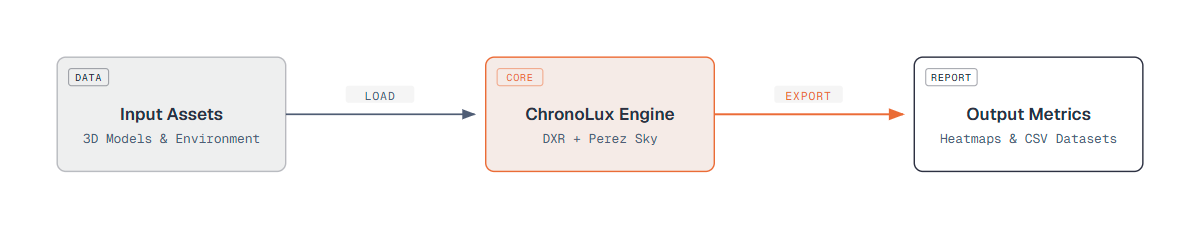
\includegraphics[width=1\textwidth]{figures/concept_diagram.png}
    \caption{High-Level Concept Architecture of the ChronoLux framework, illustrating the pipeline from raw heritage asset ingestion to real-time dosimetric data export.}
    \label{fig:concept_diagram}
\end{figure}

The subsequent chapters of this thesis will methodically detail the design, theoretical foundation, programmatic implementation, and scientific validation of these stated objectives.
 % \chapter{Project Objectives}

\chapter{Bibliographic Research}\label{ch:studiubib}

\pagestyle{fancy}


{\color{blue}\noindent This chapter should take between 3 and 10 pages.\\}

Bibliographic research has as an objective the establishment of the references for the project, within the project domain/thematic. While writing this chapter (in general the whole document), the author will consider the knowledge accumulated from several dedicated disciplines in the second semester, 4$^{th}$ year (Project Elaboration Methodology, etc.), and other disciplines that are relevant to the project theme.

Each reference \textbf{must} be cited within the document. Please look at the examples below (depending on the project theme, the presentation of a method/application can vary).

Referințele are included in the Bibliography chapter.

References can by managed with \href{https://www.jabref.org/}{JabRef}, an application which can be downloaded from \url{https://www.jabref.org/#download}

Examples of what should be included in each type of reference can be found at \href{https://libguides.nps.edu/citation/ieee-bibtex}{here}.

About common errors found in online libraries of references you can read at \href{https://www.ece.ucdavis.edu/~jowens/biberrors.html}{here}


In Chapter 4 of ~\cite{Spizner2002}, Spitzner discusses the advantages and disadvantages of honeypot systems.

References will be included in the Bibliography section. The reference format must be IEEE, or similar. The introduction of new references in the Bibliography section, and their citation within the document text can be done manually (by obeying the format), but it is not recommended as it not easy to manage them, or by using the tools mentioned in the last paragraphs of this chapter.

In the Bibliography section, there are examples of references to conferences or workshops articles ~\cite{AntoniouSBB05}, journal ~\cite{AntoniouSBDB07}, and books ~\cite{russell1995artificial}, \cite{Spizner2002}. References to applications or online resources (web pages) must include at least a short relevant description in addition to the link~\cite{seleweb}, and other information is available (authors, year, etc.). References that contain only the link to the online resource will be placed in the page footer.

Each reference must be cited within the document text, see example below (depending
on the project theme, the presentation of a method/application can vary).

%În articolul~\cite{AntoniouSBDB07} autorii prezintă un sistem pentru ...
In paper~\cite{AntoniouSBDB07} the authors present a system for moving obstacle detection using stereo-vision and an estimation of own movement.

The method is based on ... autorii prezintă un sistem pentru detecția obstacolelor în mișcare folosind stereo viziune și estimarea mișcării proprii.
Metoda se bazează pe ...\textit{discuss the algorithms, data structures, functionality, specific aspects related to the project theme, etc….} Discussion: \textit{pros and cons}.

\section{A Section Name}
\section{Another Section Name}
\subsection{A Subsection Name}
{\color{red}DO NOT copy technology descriptions here}

 % \chapter{Bibliographic Research}

\chapter{Analysis and Theoretical Foundation}\label{ch:analysis}
\pagestyle{fancy}

In this chapter, a clear definition of theoretical algorithms, mathematical abstractions, and overall logic behind the \textit{ChronoLux} design is attempted. Following the literature review, it becomes apparent that current methods of simulation suffer from significant shortcomings that render them unsuitable for application within interactive heritage metrology. Subsequently, in the following section, the theoretical measures suggested to tackle the aforementioned problems are outlined, focusing purely on abstract data manipulation and physics of light transfer.

\section{High-Level Theoretical Pipeline}\label{sec:theoretical_pipeline}
The \textit{ChronoLux} pipeline is an endless sequence of mathematical computations that turns abstract three-dimensional data into radiometric energy build-up. From an architectural perspective, the \textit{ChronoLux} system can be broken down into three separate domains. These include the Initialization Domain, Radiometric Integration Domain, and Temporal Accumulation Domain. As described earlier in Figure~\ref{fig:concept_diagram}, \textit{ChronoLux} operates on a closed-loop basis, using time-discrete iterations for its operations.

\subsection{The Initialization Domain}
Before the execution of radiometry calculations, a physical definition of the virtual environment is required. This initialization starts from the import of geometrical mesh information. From the theoretical standpoint, each artifact consists of a discrete collection of interconnected triangles forming a manifold geometry. Each of these triangles is connected to physically realistic material behavior, described by the strictly conservative thermodynamic equation ($R + T + A = 1.0$) outlined in Chapter~\ref{ch:studiubib}.

The geographical and temporal status of the simulation is established at the same time. According to the theoretical description, the coordinates of the geographic latitude ($\Phi$), geographic longitude ($\lambda$), geographic timezone offset, and the initial Julian Day of the physical heritage location are necessary inputs into the astronomy ephemeris calculation algorithm. After the completion of the first stage, a Bounding Volume Hierarchy (BVH) with a statistical optimization applied to the spatial information, as well as the solar zenith angle ($\theta_z$), and solar azimuth angle ($\gamma_s$) for the current temporal step ($t$) are derived. If the calculated solar zenith angle is less than zero ($\theta_z < 0$), then, due to the system's automatic culling mechanism, the radiometric calculation process does not have to be executed at all, moving to the next temporal iteration point.

\subsection{The Radiometric Integration Domain}
After both sets of parameters have been initialized, the system proceeds to the next stage, which is referred to as the Radiometric Integration Domain. This is where the primary mathematical algorithm for calculating irradiance takes place. Unlike in conventional rendering techniques, which use the projection of the view frustum onto the two-dimensional space, all computations take place in Texture Space, an idea that will be further explained in Section~\ref{sec:texture_space_paradigm}.

In this domain, a computational solution is sought for the Rendering Equation at all acceptable points of the artifact's surface. Rays are propagated stochastically through the hemisphere to calculate both direct sunlight and diffuse ambient light using the technique of Next Event Estimation (NEE). Directions of escaping rays are compared to the Perez All-Weather Sky Model, allowing the system to receive exact spectral values of radiance. At the end of computations, a two-dimensional grid of data that corresponds to instantaneous physical irradiance (in Lux) is obtained.

\subsection{The Temporal Accumulation Domain}
The last theoretical step comprises the constant temporal summation of the irradiance values at each moment of time. Photochemical decomposition is always an accumulative process, so the calculated radiometric information will be reused rather than thrown out after one-time processing. In particular, the instantaneous illuminance (Lux) value is multiplied by the temporal duration of the current simulation step ($\Delta t$) to derive an accumulative dosage in Lux-Hours. The accumulative dosages will be added up using a persistent floating point array. After that, the temporal counter ($t = t + \Delta t$) is advanced, and the procedure is iterated until the end of the chosen period of time (e.g., meteorological year).

\section{The Texture Space Ray Tracing Paradigm}\label{sec:texture_space_paradigm}
The first major theory in which \textit{ChronoLux} deviates from regular computer graphics is that of using the Texture Space Ray Tracing method of computation. To illustrate why such a computational method is needed in science metrology, its advantages, as well as the mathematical limitations of conventional methods, will be demonstrated below.

\subsection{The Mathematical Flaws of Screen Space Metrology}
First, in a three-dimensional engine, there is always a virtual viewer defined by a set of parameters including a field of view, distance from the screen, and near/far planes. During rendering, a two-dimensional pixel grid is used. For each pixel, there is a ray traced from the camera's optical point through the pixel into three-dimensional space.

Such an approach is mathematically exact, but it is flawed when we need to accumulate some radiation on all geometric surfaces. First, the problem is related to occlusion and perspective projection. When tracing rays from the virtual viewer, it becomes clear that the system will trace those rays that actually intersect the polygons. Any surface turned away from the viewer will not be computed because it simply will not be covered by any rays emanating from the viewer. It is obvious that if a statue is turned around the wrong way, no radiation can be accumulated on its posterior surface; the same holds true for other surfaces.

\subsection{Texture Space Mapping}
To accomplish a full separation between the simulation and the artificial restrictions of camera placement, \textit{ChronoLux} uses Texture Space Mapping. In 3D geometry, each vertex of the polygon corresponds to a point on the 2D UV plane through $(u, v)$ coordinates in three-dimensional geometry, which is called the UV map.

The process of traversing the UV map in the \textit{ChronoLux} theory does not involve traversing the pixels on the computer screen but involves traversing the discrete texels on the UV map. This allows for the recreation of geometry in world space by calculating $P$ (position) and $N$ (surface normal).

Let the UV map be a 2D matrix $M$ of size $W \times H$. For every element $M_{i,j}$:
\begin{enumerate}
    \item Read the pre-computed world-space position vector $P = (P_x, P_y, P_z)$ corresponding to the $(u, v)$ coordinate.
    \item Read the pre-computed world-space normal vector $N = (N_x, N_y, N_z)$.
    \item Use $P$ as the origin point for the dosimetric path tracer.
    \item Use $N$ to orient the sampling hemisphere.
\end{enumerate}

This method ensures that each infinitesimally small patch of the surface of the object is evaluated simultaneously, without regard to the virtual camera orientation. Global consistency of the physical light transport throughout the entire structure of the heritage object is guaranteed.

\section{Dosimetric Path Tracing Algorithm}\label{sec:dosimetric_algorithm}
For the sake of simplicity, the origin ($P$) and the direction ($N$) of the rays as established using the Texture Space technique are known; hence, it is necessary to solve the global illumination equation in order to find the exact amount of energy hitting the particular point. This task can be accomplished using a highly efficient Monte Carlo algorithm with Next Event Estimation (NEE).

\subsection{Stochastic Hemisphere Sampling and Energy Attenuation}
Firstly, to find the total irradiance on a surface, the sampling directions have to be found, which involves generating directions distributed evenly over the upper hemisphere centered at the point where the sampling takes place. Within the framework of the Monte Carlo algorithm, such distribution of samples can be represented using a stochastic directional vector $\omega_i$.

To improve convergence rates and minimize variance, \textit{ChronoLux} uses Cosine-Weighted Importance Sampling. Instead of uniformly sampling random vectors, the probability density function used here tilts towards the vertical axis that passes through the surface normal. This method mirrors the physics behind lambertian diffuse surfaces when light coming from the vicinity of the surface normal carries more energy (proportional to $\cos(\theta)$) than that coming in from a large angle $\theta$.

As these stochastic rays traverse the digital scene, they interact with other surfaces. The core principle behind this interaction is energy absorption, meaning the photonic path will dissipate its energy after each encounter with another surface. Thus, an object placed in a room with dark mahogany walls (with high Absorptance, $A$) will reflect indirect rays with significantly less energy than those reflected from white plaster (high Reflectance, $R$).

This effect can be easily modelled mathematically through the use of a throughput multiplier. Starting with an initial value of 1.0, which means perfect energy transmission, throughput gets multiplied by Reflectance $R$ at each encounter. As $R < 1.0$ for any physical surface (following the law of conservation of energy $R + T + A = 1.0$), the ray loses energy at an exponential rate after each reflection.

In order to prevent simulation from becoming infinitely long, because of an endless number of bounces in enclosed space, a finite bounce depth limit should be set. For example, typical indirect path lengths do not exceed 3 or 4 bounces since additional reflections carry too little residual energy to matter further.

\subsection{The Physics of Refractive Transmission}
A basic element of heritage metrology involves evaluating the impact of external light that passes through physical obstacles, especially the effects of window glazing. This requires realistic modeling of refraction for light.

When a path traced ray meets a boundary between two media (say, a pane of glass), the ray does not necessarily stop or bounce off. Rather, it changes direction based on the IORs of the two media (air-glass) according to Snell's Law:

\begin{equation}
    \frac{\sin \theta_1}{\sin \theta_2} = \frac{n_2}{n_1}
\end{equation}
In the above-mentioned framework, $n_1$ and $n_2$ stand for the refractive indices of the media from which the ray starts and where it reaches, respectively; while $\theta_1$ and $\theta_2$ stand for the angles of incidence and refraction, respectively, regarding the normal to the interface.

As far as the \textit{ChronoLux} abstract model is concerned, the transmission vector is calculated via Snell's Law whenever the beam penetrates a transparent body, allowing the ray to proceed with its travel through the solid glass. At the same time, the throughput of the ray is adjusted with respect to the particular material's Transmittance ($T$) factor. If a conservator applies UV-blocking film with a Transmittance of 0.45, the ray throughput is immediately decreased by 55\%, thus providing an adequate simulation of the real-world effect produced by the intervention.

\subsection{Next Event Estimation (NEE)}

In a pure Monte Carlo path tracer, all sampling is random, and the tracing algorithm can use only random reflection from surfaces. The chance of finding the sun's small angular diameter through random reflections inside a dark museum is practically nil; therefore, there is significant variance in the simulation, and one would need to calculate millions of samples to converge toward the correct answer, rendering the calculation unfeasible at least with respect to the 8,760-hour simulation.

To alleviate this problem, \textit{ChronoLux} employs the technique known as Next Event Estimation (NEE).

At every single interaction point $P$ across the entire bounce sequence, the algorithm performs the following logic:
\begin{enumerate}
    \item \textbf{Direct Shadow Ray:} A deterministic vector $\omega_{sun}$ is generated with the direction towards the exact current location of the sun. "Shadow ray" tracing occurs along $\omega_{sun}$. If this ray leaves the bounded region without intersection with any opaque objects, the direct irradiance is calculated using the Perez model and added to the total dose. In case there is an intersection with a transparent object (such as window glass), the light intensity will be reduced by a factor of $T$ which is obtained using Snell's law.
    \item \textbf{Indirect Bounce Ray:} At the same time, a stochastic vector $\omega_i$ is generated using Cosine-Weighted Importance Sampling. Tracing is performed along this vector to calculate the indirect light caused by reflection from walls and floors.
\end{enumerate}

Through its clear disentanglement of the deterministic solar irradiance and the random scattering of the ambient sky dome, NEE guarantees that the massive energy content of the sun is properly accounted for at every stage of the simulation, thus reducing the number of samples needed by many orders of magnitude and ensuring metrological stability. The total irradiance of the starting surface point is thus computed as the sum of all successful shadow rays cast from the initial surface point through multi-bounces.

\subsection{Miss Evaluation and Perez Integration}
The last piece of the integration domain puzzle is that of Miss evaluation. When the stochastic ray (be it the direct shadow ray or the indirect bounced ray) finally escapes the digital twin architecture, it will need to retrieve the radiance value from the physical world surrounding the building.

Contrary to returning a hardcoded color, the escaping ray direction, $\omega_{escape}$, is mathematically inserted into the Perez All-Weather Sky Model function. This function calculates the elevation ($\theta_z$) and azimuth ($\gamma_s$) of $\omega_{escape}$ against the current solar location ($\theta_z$, $\gamma_s$) and uses the meteorological data of Clearness ($\epsilon$) and Brightness ($\Delta$) to calculate the physical luminance value of $\omega_{escape}$. If $\omega_{escape}$ happens to be near the solar disk, the result will undergo an exponential increase to simulate the Mie circumsolar scattering effect. Otherwise, if $\omega_{escape}$ is close to the horizon, then the Perez output transitions smoothly to simulate Rayleigh scattering.

\section{The Parallel Determinism Problem}\label{sec:parallel_determinism}
One of the problems that arises when moving from the abstract realm of mathematics into practical implementations in highly parallel architectures, such as today's GPUs, is non-determinism in floating-point additions.

A typical parallel tracing algorithm traces hundreds of millions of rays independently using thousands of threads simultaneously. Once the rays finish traversing the scene, all threads attempt to write their irradiance into a shared matrix of accumulations $M$.

As opposed to integer numbers, floating-point operations are non-associative, meaning that $(A + B) + C \neq A + (B + C)$ because of tiny differences that occur during precision rounds in IEEE 754. As a result, the final value of luminance will be different each time the algorithm runs if the order of writing to the accumulation matrix $M$ by the threads is random.

In video games, this minute difference is not detectable. When applied to science, however, non-determinism becomes unacceptable since an analysis tool must return the same results every time a test simulation is conducted.

The solution to the problem for the \textit{ChronoLux} framework involves making sure that ray tracing is done and accumulations happen in a predetermined manner, through mathematical structuring of geometry or seed points. This solution may add minimal computational expense, but it guarantees mathematical consistency and reproducibility.

\section{Mathematical Dose Accumulation}\label{sec:dose_accumulation}
The key theoretical objective of the \textit{ChronoLux} tool is not only creating a photographically accurate representation of light but rather finding the overall photochemical risk posed over a long period of time. It implies moving from considering an instantaneous value of illumination to a cumulative dosimetry one.

\subsection{Temporal Integration Logic}
Let $E_t(P)$ be the instantaneous physical irradiance (measured in Lux) estimated with the help of dosimetric path tracer on a particular surface point $P$ in a particular moment of time $t$.

Light illumination in a physical museum is a continuous process, while a digital simulation has to discretize time into particular segments ($\Delta t$). The choice of $\Delta t$ significantly affects not only the accuracy of the calculation but also its performance. A traditional meteorological simulation usually takes 1 hour for each $\Delta t$. It allows tracking a motion of the Sun and cloud cover change in 8,760 steps within a typical year.

Cumulative dose $D(P)$ delivered to a particular surface point $P$ for the whole period of time $T$ is theoretically equal to the following sum:

\begin{equation}
    D(P) = \sum_{t=0}^{T} E_t(P) \cdot \Delta t
\end{equation}

Where:
\begin{itemize}
    \item $D(P)$ is the total accumulated exposure in Lux-Hours.
    \item $E_t(P)$ is the calculated irradiance in Lux at time step $t$.
    \item $\Delta t$ is the duration of the time step in hours.
\end{itemize}

\subsection{Floating-Point Precision and Heatmap Generation}
In order to retain the accumulating radiation dosage $D(P)$, the program uses the previously discussed Texture Space $M$ matrix. Standard bitmap file formats (such as the 8-bit PNG or JPEG) cannot be used to store dosimetric data, as they can only store values from the set of integers ranging from 0 to 255. An extremely sensitive piece of art may amass as much as 50,000 Lux-Hours during its lifetime, which will quickly surpass the capacity of the 8-bit variable.

Therefore, according to the theory, the system makes use of a 32-bit floating point data structure (RFloat). A 32-bit float can theoretically encode $3.4 \times 10^{38}$, providing practically infinite precision for unbounded accumulation.

As the simulation advances within the temporal dimension, the matrix elements continuously increase in value. The abstract mathematical information is then mapped to a heatmap for visual analytical representation of areas where photosensitivity risks are critical.

\section{Conclusion}
Thus, in conclusion, the theories described in the current chapter make \textit{ChronoLux} a purely metrological simulation software. Abandoning the bias-laden approach of the Screen Space rendering in favor of the Texture Space ray tracing method guarantees complete geometrical coverage. Furthermore, Next Event Estimation, together with the Perez Sky Model algorithm, ensures exact computation of the light transport. Finally, accumulating irradiation in an arbitrarily precise floating point matrix allows for accurate simulation of photochemical degradation for meteorological years. % \chapter{ Analysis and Theoretical Foundation}

\chapter{Detailed Design and Implementation}
\pagestyle{fancy}

This chapter provides an exhaustive breakdown of the software engineering architecture, the hardware-accelerated algorithms, and the rigorous mathematical systems implemented to realize the \textit{ChronoLux} digital twin. Transitioning from theoretical radiometry and conservation physics into a highly performant desktop application requires a sophisticated orchestration of CPU scheduling, unmanaged memory transfers, and massive GPU parallelization. 

Predictive analysis workflows governed by the International Commission on Illumination (CIE) and Michalski guidelines for preventive conservation historically suffer from a lack of interactivity. Traditional offline software like Radiance demands hours of CPU-bound calculations for a single temporal simulation. \textit{ChronoLux} resolves this bottleneck by implementing a hybrid architecture utilizing the Unity 3D engine and the DirectX 12 graphics API to unlock hardware-accelerated DirectX Raytracing (DXR). This chapter systematically dissects each component of this pipeline, from mathematical astrometry to GPU memory management and asynchronous telemetry extraction.

\section{Software Architecture Overview}

To process the massive volume of ray queries required for an annual dosimetric simulation without halting the operating system, a strictly decoupled architecture is employed. The software stack is bifurcated into two distinct domains: the C\# CPU layer handling user interface, file I/O, deterministic structural sorting, and astrometric mathematics; and the HLSL Compute Shader layer executing the heavily parallelized Monte Carlo integrations directly on the GPU.

\begin{figure}[htbp]
	\centering
	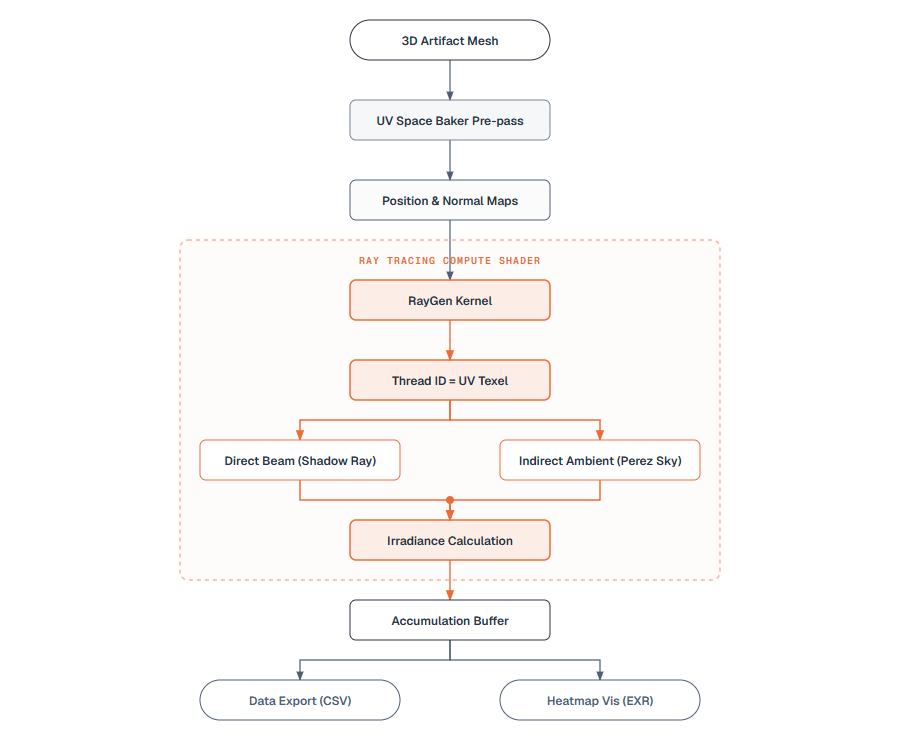
\includegraphics[width=\textwidth]{figures/pipeline.png}
	\caption{High-level simulation pipeline demonstrating the decoupling of CPU orchestration from GPU execution.}
	\label{fig:pipeline_diagram}
\end{figure}

\begin{figure}[htbp]
	\centering
	
\includegraphics[width=\textwidth]{figures/architecture.png}
	\caption{Overall Architectural System design of \textit{ChronoLux}, detailing data paths between the Engine, the GUI, and the OS filesystem.}
	\label{fig:architecture_diagram}
\end{figure}

As seen in Figures \ref{fig:pipeline_diagram} and \ref{fig:architecture_diagram}, the flow of data is strictly managed. Project parameters are serialized to JSON via the \texttt{ChronoProject} object, parsed by the \texttt{ProjectManager}, and fed into the \texttt{LightDoseSimulator}. This orchestrator acts as the simulation's beating heart, stepping time forward and delegating ray dispatching to the DXR kernels.

\section{Core Simulation Engine (C\# CPU Orchestration)}

The core logic of the application must ensure mathematical determinism, prevent hardware starvation, and respond dynamically to user inputs.

\begin{figure}[htbp]
	\centering
	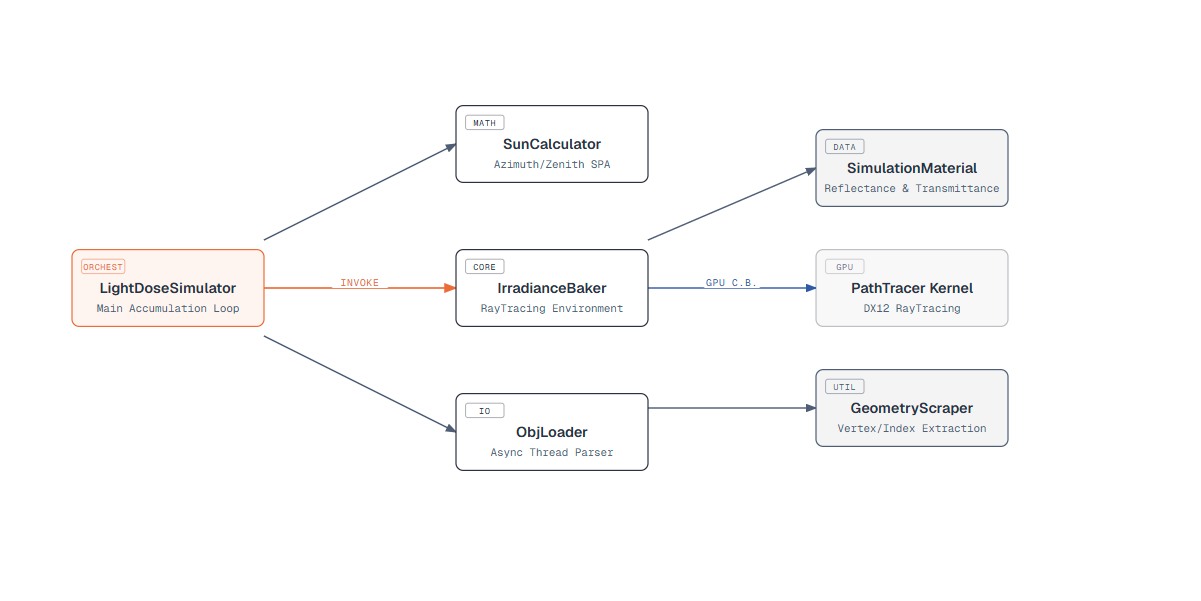
\includegraphics[width=\textwidth]{figures/csharp_class_diagram.png}
	\caption{C\# CPU Class Architecture and Data Flow orchestration within \textit{ChronoLux}.}
	\label{fig:csharp_class_diagram}
\end{figure}

As shown in Figure \ref{fig:csharp_class_diagram}, the \texttt{LightDoseSimulator} depends on several critical sub-systems: \texttt{SunCalculator} for astrometric mathematics, \texttt{IrradianceBaker} for hardware dispatching, and \texttt{RuntimeModelLoader} for asynchronous file I/O.

\subsection{The Chronological Engine and Time Stepping}

The primary responsibility of the \texttt{LightDoseSimulator} is to advance the master clock $\Delta t$ and generate the precise solar altitude and azimuth required for the Perez sky model. 

The simulation logic must process an entire meteorological year while preventing the Operating System from triggering a Timeout Detection and Recovery (TDR) crash, which forcefully restarts the graphics driver if a single task takes longer than approximately 2 seconds. This is achieved via a C\# \texttt{IEnumerator} Coroutine (\texttt{RunSimulationInternal}). As detailed in Appendix \ref{apx:csharp_code} (Listing \ref{lst:timeloop}), the time-stepping loop is entirely dynamic. It processes the user-defined \texttt{startDay} and \texttt{endDay} linearly. 

For every single day, the Coroutine utilizes the \texttt{SunCalculator} to dynamically query the exact local sunrise and sunset boundaries based on the user's defined latitude, longitude, and UTC offset. This prevents the simulation from wasting cycles tracing rays in the middle of the night. If the calculated sunrise and sunset times are identical (an edge case during polar nights at extreme latitudes), the simulation intelligently skips the entire day.

An aggressive computational culling strategy is further employed inside the hourly step loop. The engine skips any temporal step where both the incoming direct beam lux and the diffuse sky lux are calculated to be functionally zero (specifically $< 0.1$ Lux). By omitting these low-energy twilight steps where atmospheric scattering absorbs nearly all solar irradiance, \textit{ChronoLux} saves millions of unnecessary Monte Carlo ray casts per simulated year, directly boosting overall performance. 

During active simulation periods, the Coroutine explicitly uses the \texttt{yield return null;} statement. This instruction pauses the Coroutine's execution until the next engine frame, actively yielding the thread back to the Unity main loop. This guarantees that the UI remains fully responsive, the progress bar animates smoothly, and the TDR watchdog is appeased.

\subsection{Mathematical Astrometry and Solar Ephemeris}

Achieving metrological accuracy requires precise solar positioning at every hour of the year. The \texttt{SunCalculator.cs} class implements rigorous celestial mathematical models, determining not only the vector position of the solar disc but also evaluating atmospheric attenuation to yield physically accurate \texttt{BeamLux} and \texttt{DiffuseLux} values.

The first step converts the local simulation time into a Julian Day (JD) epoch, calculating Julian centuries $T$ from J2000.0. The geometric mean longitude ($L_0$) and mean anomaly ($M$) of the sun are given by:
\begin{equation}
L_0 = \left(280.46646 + T(36000.76983 + T \times 0.0003032)\right) \pmod{360^\circ}
\end{equation}
\begin{equation}
M = 357.52911 + T(35999.05029 - 0.0001537 \times T)
\end{equation}

To account for Earth's orbital eccentricity, the Equation of Center ($C$) is derived using Fourier series expansion, which corrects the geometric mean longitude to the apparent longitude ($\lambda_{app}$):
\begin{equation}
C = \sin(M)(1.914602 - 0.004817 T) + \sin(2M)(0.019993) + \sin(3M)(0.000289)
\end{equation}

The Mean Obliquity of the Ecliptic ($\epsilon_0$) is corrected for nutation to calculate the Solar Declination ($\delta$), defining how far the sun resides above or below the celestial equator:
\begin{equation}
\delta = \arcsin\left(\sin(\epsilon) \sin(\lambda_{app})\right)
\end{equation}

With $\delta$ established, the Equation of Time ($EqT$) maps solar time to clock time. Combining $EqT$ with the terrestrial longitude yields the True Solar Time (TST) and the Hour Angle ($H$):
\begin{equation}
H = \frac{TST}{4.0} - 180^\circ
\end{equation}

Finally, the Solar Zenith Angle ($\theta_z$) and Azimuth ($\phi$) are strictly defined relative to the user's latitude ($\Phi$):
\begin{equation}
\cos(\theta_z) = \sin(\Phi)\sin(\delta) + \cos(\Phi)\cos(\delta)\cos(H)
\end{equation}

With the astrometric vector position fixed, the clear-sky direct beam irradiance ($E_{beam}$) is computed using the rigorous Kasten-Young formula for optical air mass ($AM$). As the sun approaches the horizon, the thickness of the atmosphere the light must penetrate increases non-linearly:
\begin{equation}
AM = \frac{1}{\sin(\alpha) + 0.50572(\alpha + 6.07995)^{-1.6364}}
\end{equation}
\begin{equation}
E_{beam} = 127500 \times 0.7^{AM^{0.678}} \quad [\text{Lux}]
\end{equation}
Where $\alpha$ is the solar altitude angle ($90^\circ - \theta_z$), and $0.7$ acts as the baseline atmospheric transmittance coefficient for clear-sky conditions.
For ambient lighting, a simplified Haurwitz clear-sky diffuse model calculates horizontal diffuse illuminance ($E_{diffuse}$), estimating atmospheric scattering based on the total potential solar constant versus direct atmospheric penetration. These precise \texttt{BeamLux} and \texttt{DiffuseLux} values are injected directly into the HLSL compute kernel for every single time step.

\section{Scene Management and Hardware Interfaces}

\subsection{Asynchronous Runtime Mesh Parsing}

Because \textit{ChronoLux} is distributed as a compiled desktop metrology application, it cannot rely on pre-compiled Unity Scene assets. It must dynamically load arbitrary, user-provided \texttt{.obj} files at runtime from the local filesystem. Heritage artifacts, such as laser-scanned church interiors or high-resolution photogrammetry models, can easily exceed several million vertices. If a string-based parser attempted to read these files synchronously on the main Unity thread, the application would permanently freeze, and the OS would terminate it with an "Application Not Responding" failure.

As demonstrated in Appendix \ref{apx:csharp_code} (Listing \ref{lst:objloader}), the \texttt{RuntimeModelLoader.cs} resolves this memory bottleneck by implementing a heavily threaded chunk parser. The reading of the file and the string parsing of vertices, normals, and UV coordinates occurs entirely inside a \texttt{Task.Run()} background thread executing on separate logical CPU cores. 
While this parse task runs in the background, the main thread loop evaluates a \texttt{while (!parseTask.IsCompleted)} condition, repeatedly calling \texttt{yield return null;} and updating the \texttt{ProgressBar} UI element via \texttt{UpdateProgress()}. Only once the massive memory arrays are fully populated is execution yielded back to the Unity main thread for the final \texttt{Mesh.SetVertices()} upload to VRAM and the subsequent \texttt{GameObject} generation. This architecture keeps the UI fully responsive during the heaviest data loads.

\subsection{Dynamic Material Serialization and Hierarchy Keying}

When a heritage artifact is loaded via the runtime loader, the original materials are completely stripped. Instead, the simulation maps physically validated presets (e.g., Brick, Hardwood, Antique Glass) onto the individual sub-meshes. This mapping is securely persisted in the \texttt{ChronoProject} JSON file.

To re-apply these materials safely across different application sessions, the \texttt{RuntimeModelLoader} uses a unique string keying mechanism. Relying purely on a \texttt{GameObject}'s name is insufficient because `.obj` files often contain duplicate component names like \texttt{Wall} or \texttt{Window\_01}. The \texttt{GetObjectKey} function constructs a distinct hierarchical identifier:
\begin{lstlisting}[language={[Sharp]C}]
private string GetObjectKey(GameObject go) {
    if (go.transform.parent != null && go.transform.parent != modelRoot)
        return $"{go.transform.parent.name}/{go.name}";
    return go.name;
}
\end{lstlisting}
This \texttt{RootName/MeshName} composite key guarantees that when the \texttt{ApplySavedMaterial} logic iterates over the loaded mesh components, it securely matches the geometry against the serialized \texttt{project.objectNames} array and retrieves the exact GUID for the \texttt{project.materialPresetNames}, completely avoiding material crossover errors.

\subsection{Spatial Normalization}

Imported geometries exhibit extreme variations in scale; some architectural models are constructed in millimeters, others in meters, and some geographic surveys in kilometers. To prevent catastrophic floating-point precision loss inside the DXR kernel—which occurs when rays must intersect extremely large coordinate spaces—\textit{ChronoLux} applies a strict spatial normalization pipeline via the \texttt{CenterAndScaleModel} function.

The algorithm calculates the global bounding box encapsulating all sub-meshes attached to the artifact root. It determines the maximum dimensional span:
\begin{equation}
MaxDim = \max(Width, \max(Height, Depth))
\end{equation}
A uniform scaling factor is then calculated: $Factor = 2.0 / MaxDim$ (assuming $MaxDim > 0$). Every child vertex transform is then translated so the object's mathematical centroid rests exactly at local $(0,0,0)$, and scaled uniformly by the $Factor$. This mathematical normalization guarantees that the entire heritage site, regardless of its original CAD scale, strictly occupies a 2.0-meter bounding box in World Space. 
Because the DXR ray tracer relies on 32-bit floating point math, keeping intersection geometry strictly within the $[-1.0, 1.0]$ bounds near the origin maximizes the IEEE 754 mantissa precision, preventing "shadow acne" and geometric clipping. The user's semantic transformations (position and scale offsets loaded from the \texttt{ChronoProject} JSON) are then applied exclusively to the normalized root object.

\subsection{Deterministic BVH Building}

As highlighted in theoretical radiometry literature, Monte Carlo integration is susceptible to floating-point associativity errors. However, an even greater threat in a hybrid CPU-GPU engine is structural non-determinism. Unity's \texttt{FindObjectsByType<Renderer>()} API does not guarantee a strictly deterministic return order across different operating systems or CPU architectures. If the mapping between a ray's geometric \texttt{InstanceID} and its underlying physical \texttt{SimulationMaterial} shifts between runs, the dosimetric simulation loses all scientific reproducibility.

To resolve this, the \texttt{IrradianceBaker.cs} initialization enforces strict determinism by collecting all active \texttt{Renderer} components and explicitly sorting them using a deeply granular $O(n \log n)$ string-based ordinal comparison. The unique \texttt{SortKey} for every sub-mesh is constructed as follows:
\begin{equation}
\text{SortKey} = \text{ScenePath} \,|\, \text{TransformHierarchy} \,|\, \text{Type} \,|\, \text{MaterialSlot}
\end{equation}
The \texttt{TransformHierarchy} is built by recursively ascending the parent tree and appending the exact \texttt{GetSiblingIndex()} padded to 6 digits (e.g., \texttt{000002:Wall/000000:Window}). This incredibly stable ordinal sort guarantees that the structural Index and Vertex buffers uploaded to the GPU, alongside the \texttt{\_SimulationMaterials} \texttt{StructuredBuffer}, are mathematically identical and perfectly aligned across entirely different hardware platforms, ensuring absolute reproducibility in lux-hour accumulation.

\section{Hardware-Accelerated Path Tracing (HLSL / DXR)}

The true computational bottleneck of \textit{ChronoLux} lies within the ray tracing logic. For every pixel in the artifact's UV map, stochastic rays must be cast to evaluate the rendering equation over thousands of simulated hours.

\subsection{Memory Management and DXR Acceleration Structures}

DirectX Raytracing relies on a hardware-accelerated two-tier hierarchy: the Bottom-Level Acceleration Structure (BLAS) storing raw triangle data, and the Top-Level Acceleration Structure (TLAS) defining spatial instances of the BLAS. In \textit{ChronoLux}, the TLAS is built and managed via Unity's \texttt{RayTracingAccelerationStructure}. 

Memory is strictly managed to align with GPU 16-byte boundaries. Data blocks transferred to the graphics card must obey HLSL packing rules to prevent memory corruption. For example, the \texttt{MeshMetadata} struct is explicitly padded inside C\# to ensure an exact 16-byte footprint:
\begin{lstlisting}[language={[Sharp]C}]
[StructLayout(LayoutKind.Sequential)]
private struct MeshMetadata {
    public uint vertexOffset;  // 4 bytes
    public uint indexOffset;   // 4 bytes
    public uint hasGeometry;   // 4 bytes
    public uint padding;       // 4 bytes (Forcing 16-byte alignment)
}
\end{lstlisting}
Similarly, the GPU expects \texttt{float4} structures for optimal SIMD (Single Instruction, Multiple Data) processing lanes. As a result, the \texttt{\_NormalMap} texture utilizes all four channels, storing the geometric $(x,y,z)$ coordinates in the RGB channels, while reserving the alpha channel ($w$) as a strictly binary coverage flag indicating valid geometry versus empty padding space.

The \texttt{SimulationMaterial} variables (reflectance, transmittance) are packed into \texttt{Vector4} arrays and mapped into the \texttt{\_SimulationMaterials} \texttt{ComputeBuffer}. When the \texttt{IrradianceBaker} builds the TLAS using \texttt{rtas.AddInstance()}, it applies specific flags. Sub-meshes are assigned \texttt{RayTracingSubMeshFlags.ClosestHitOnly}. This hardware optimization disables the invocation of "Any-Hit" shaders during traversal, significantly improving silicon performance since the simulation only requires the absolute nearest geometric intersection point.

\begin{figure}[htbp]
	\centering
	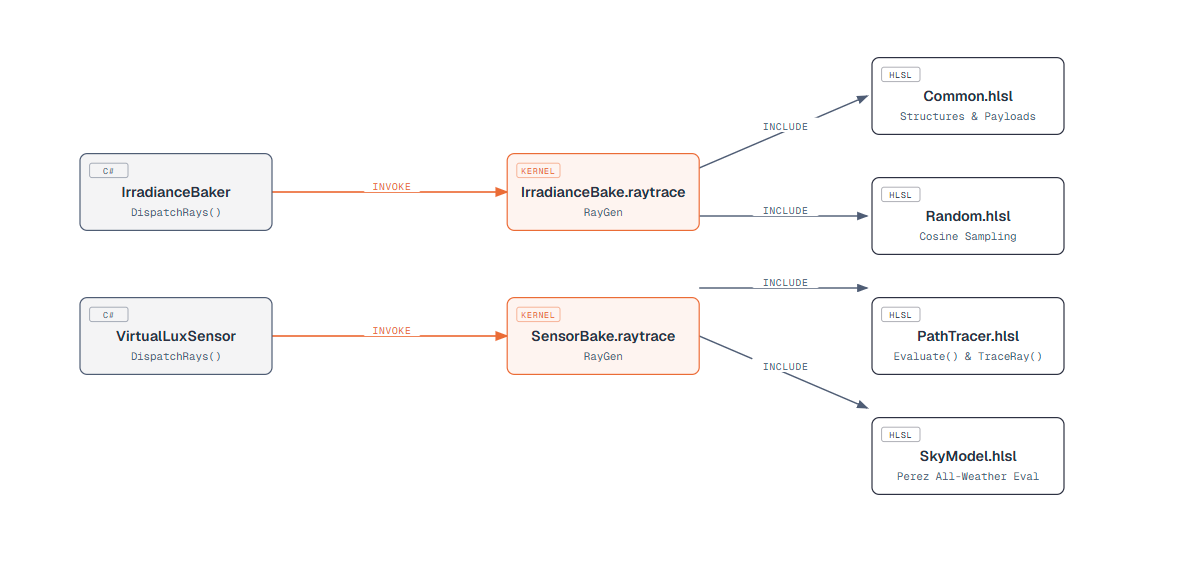
\includegraphics[width=\textwidth]{figures/shader_class_diagram.png}
	\caption{HLSL Compute Shader modular structure and inclusion tree.}
	\label{fig:shader_class_diagram}
\end{figure}

\subsection{Texture Space Dispatch Paradigm}

\textit{ChronoLux} drastically diverges from traditional screen-space video game graphics by utilizing Texture Space Ray Tracing. Instead of firing primary rays from the user's virtual camera lens towards a 1080p screen grid (which would only accumulate dose for pixels currently visible to the user), the compute kernel maps threads directly to the two-dimensional $(u,v)$ coordinates of the target mesh's unrolled UV layout.

\begin{figure}[H]
    \begin{algorithmic}
        \Require $PosMap, NormMap, SunDir, N_{samples}, \Delta t$
        \For{\textbf{each} thread $id \in \text{DispatchThreadID}$}
        \State $\mathbf{p} \leftarrow PosMap[id].xyz$
        \State $\mathbf{n} \leftarrow NormMap[id].xyz$
        \If{$\text{length}(\mathbf{n}) < 0.1$}
        \State \textbf{return} \quad \text{// Terminate thread (empty UV padding)}
        \EndIf
        
        \State $E_{dir} \leftarrow 0$
        \State $NdotL \leftarrow \mathbf{n} \cdot SunDir$
        \If{$NdotL > 0.0$}
        \State $E_{dir} \leftarrow \textsc{TracePath}(\mathbf{p}, SunDir, \dots, \text{isDirectSun=true}) \times NdotL$
        \EndIf
        
        \State $E_{ind} \leftarrow 0$
        \For{$i = 1$ \textbf{to} $N_{samples}$}
        \State $\omega_i \leftarrow \textsc{GetCosineWeightedDirection}(\mathbf{n})$
        \State $E_{ind} \leftarrow E_{ind} + \textsc{TracePath}(\mathbf{p}, \omega_i, \dots, \text{isDirectSun=false})$
        \EndFor
        
        \State $E_{total} \leftarrow E_{dir} + (E_{ind} / N_{samples}) \cdot \pi$
        
        \State $DoseMap[id] \leftarrow DoseMap[id] + E_{total} \cdot \Delta t$
        \State $DirectDoseMap[id] \leftarrow DirectDoseMap[id] + E_{dir} \cdot \Delta t$
        \State $IndirectDoseMap[id] \leftarrow IndirectDoseMap[id] + (E_{ind} / N_{samples}) \cdot \pi \cdot \Delta t$
        \EndFor
    \end{algorithmic}
    \caption{Pseudocode for Texture Space Ray Tracing dispatch separated into Direct and Stochastic Multi-Sampling paths.}
    \label{alg:ts_raytrace}
\end{figure}

A pre-pass baker uses the standard rasterization pipeline to write the world-space positions ($P$) and geometric normals ($N$) into \texttt{\_PositionMap} and \texttt{\_NormalMap} textures. As shown in Algorithm \ref{alg:ts_raytrace} (and detailed in Appendix \ref{apx:pathtracer_code}), the ray generation kernel (\texttt{IrradianceBakeRayGen}) is dispatched across this 2D grid. If a pixel has a normal length near zero, it indicates empty void space in the UV padding, and the thread terminates instantly to save cycles. Otherwise, the kernel uses $P$ and $N$ as the origin and orientation for the evaluation of the rendering equation. This architecture makes light simulation completely detached from screen space, permanently baking energy data directly onto the architectural surface.

\subsection{Pseudo-Random Sequence Generation and Hashing}

Monte Carlo integration fundamentally relies on uniform random sampling across the target domain (the celestial hemisphere). If the random number generator exhibits clustering or spatial-temporal correlations, the rendering equation evaluation becomes biased, manifesting as structural noise patterns rather than a uniform reduction in variance.

To resolve this inside the HLSL kernel without the overhead of tracking massive state arrays, \textit{ChronoLux} implements a stateless hashing algorithm bound to the thread's pixel coordinate ($x, y$) and the active simulation time step ($\Delta t$). 
\begin{equation}
\text{baseSeed} = \text{Hash}(id.y \times \text{dims}.x + id.x + \text{\_FrameIndex})
\end{equation}
By directly injecting \texttt{\_FrameIndex} (a sequentially increasing integer tracking the specific temporal step) into the core integer hash, the generated sequence of stochastic multi-samples shifts continuously throughout the year. As hundreds of time steps accumulate into the single \texttt{\_DoseMap} buffer, the high-frequency noise mathematically cancels itself out, allowing the Monte Carlo estimator to organically converge towards the true ground-truth irradiance integral.

\subsection{Direct Sunlight and Stochastic Multi-Sampling Paths}

To accurately evaluate the ambient light bouncing through the environment, \textit{ChronoLux} distinctly splits the integration into two explicit paths inside the ray generation shader.

The first path handles \textbf{Direct Sun}. If the surface normal faces the solar vector (\texttt{nDotSun > 0.0}), a single specific ray is fired directly towards the analytical sun vector by calling \texttt{TracePath} with \texttt{isDirectSun = true}. Inside \texttt{PathTracer.hlsl}, direct rays are uniquely allowed to traverse through transparent geometry. If the direct ray hits a material, the hardware queries the \texttt{\_SimulationMaterials} buffer for \texttt{transmittance}. If transmittance is greater than zero (e.g., stained glass), the throughput multiplier is attenuated by the transmittance value, the ray origin is nudged explicitly forward, and the ray continues its traversal through the object towards the sun. If transmittance is zero, it acts as an opaque shadow caster, and the traversal immediately returns $0.0$ lux.

The second path handles \textbf{Indirect Ambient Bouncing} via Stochastic Multi-Sampling. For every pixel, a \texttt{for}-loop generates $N_{samples}$ pseudo-random vectors over the hemisphere utilizing Cosine-Weighted Importance Sampling (\texttt{GetCosineWeightedDirection}). These rays call \texttt{TracePath} with \texttt{isDirectSun = false}. 

Unlike direct rays, indirect rays utilize the probabilistic \textbf{Russian Roulette} path termination technique. Russian Roulette provides an unbiased mathematical framework for terminating infinite recursive bounces without arbitrarily clipping light energy. At each bounce intersection, a random float $rv \in [0, 1)$ is generated from the hash sequence. Based on the material's scalar \texttt{reflectance} ($R$) and \texttt{transmittance} ($T$), the ray's fate is decided via cumulative probability thresholds:
\begin{enumerate}
    \item \textbf{Reflection ($rv < R$)}: The ray survives and generates a new cosine-weighted hemisphere vector.
    \item \textbf{Transmission ($rv < R + T$)}: The ray passes directly through the surface geometry without deviating its trajectory.
    \item \textbf{Absorption ($rv \geq R + T$)}: The ray is probabilistically absorbed by the material, and the path is immediately terminated.
\end{enumerate}

Because the ray only continues its trajectory when it mathematically "survives" the material's properties, the throughput does not need to be manually divided by the reflection multiplier at every vertex—the probability of survival itself acts as the exact energy attenuation weighting factor. If an indirect ray escapes the bounding volume hierarchy (BVH) without being fully absorbed, it triggers the \texttt{EvaluateSky()} function, tapping into the Perez Sky Model to fetch physically accurate atmospheric luminance. This deeply recursive behavior allows \textit{ChronoLux} to accurately calculate highly occluded indirect lighting scenarios, such as light bouncing down a hallway or reflecting off a highly reflective marble floor onto a textile artifact.

\section{Advanced Mathematical Models and Optimization}

To ensure the scientific validity and computational feasibility of the simulation, several advanced mathematical paradigms and hardware optimizations are integrated into the \textit{ChronoLux} engine.

\subsection{Perez Sky Model Atmospheric Coefficients}

While the direct solar disc dictates the intense beam irradiance, the vast majority of complex architectural ambient lighting is driven by diffuse sky scattering. \textit{ChronoLux} evaluates this using the Perez All-Weather Sky Model (\texttt{SkyModel.hlsl}), which models the highly anisotropic luminance of the celestial dome.

The engine implements the model for a clear sky with a Turbidity of $T=2.0$, utilizing five empirically derived static coefficients:
\begin{itemize}
    \item $a = -0.1058$: Dictates horizon brightening or darkening.
    \item $b = -0.0738$: Controls the luminance gradient near the horizon.
    \item $c = 1.8200$: Defines the relative intensity of the circumsolar corona.
    \item $d = -2.9744$: Controls the spatial width of the circumsolar region.
    \item $e = 0.1778$: Defines the backward scattered light opposing the sun.
\end{itemize}

Whenever an indirect stochastic ray misses all geometry, the zenith angle ($\theta$) and the angular distance to the sun ($\gamma$) are calculated. The relative luminance is evaluated via the scattering indicatrix function:
\begin{equation}
f(\theta, \gamma) = \left[1 + a \exp\left(\frac{b}{\cos\theta}\right)\right] \times \left[1 + c \exp(d \gamma) + e \cos^2\gamma\right]
\end{equation}
The result is then normalized against the dynamically calculated \texttt{DiffuseLux} provided by the CPU astrometry system (via the normalization factor $E_{diffuse} \times 0.2$). This evaluates to a physically accurate spectral distribution that perfectly mimics real-world atmospheric scattering.

\subsection{Hardware Traversal Mechanics (DXR and Face Culling)}

The decision to build \textit{ChronoLux} strictly upon DirectX 12 DXR fundamentally shifts the traversal bottleneck from software to raw silicon. Modern desktop GPUs feature dedicated Ray Tracing Cores that natively accelerate the traversal of the BVH tree and the complex Moeller-Trumbore ray-triangle intersection mathematical tests.

Furthermore, when the \texttt{TraceRay} HLSL intrinsic is called for direct sunlight shadows, a specific ray flag is injected into the payload structure: \texttt{RAY\_FLAG\_CULL\_BACK\_FACING\_TRIANGLES}. Because direct shadow rays only care about binary occlusion (is the sun visible or blocked?), and since architectural CAD models are typically closed manifolds (e.g., a wall has two sides), this hardware flag immediately discards intersection tests against any triangle facing away from the ray origin. This halves the computational burden on the RT Cores for shadow evaluation. Crucially, this optimization is explicitly disabled for indirect multi-bounce rays, as light must be able to reflect off the interior back-faces of transparent geometry like display cases.

\section{Asynchronous Data Telemetry and UI Integration}

\subsection{Automated Sensor Placement}

In physical metrology, scientists place physical lux meters around the laboratory. In the digital twin, \textit{ChronoLux} mimics this behavior by deploying \texttt{VirtualLuxSensor} objects. 
To guarantee objective baseline measurements, the \texttt{RuntimeModelLoader} automates the placement of an outdoor reference sensor array. When an environment model is loaded, the engine invokes \texttt{CreateOutdoorReferenceSensors}. This function iterates across all renderers to calculate a global master bounding box enclosing the entire heritage site. It derives the highest spatial point ($Y_{max} + 2.0\text{m}$) and the total geometric radius. Five sensors are then spawned automatically—one directly in the center, and four arranged in a complete perimeter circle. This ensures that regardless of the complexity of the CAD artifact below, there will always be unobscured sensors tracking the unadulterated baseline sunlight potential for that specific latitude and day.

\subsection{Metrological Analytics Pipeline}

True scientific metrology requires raw, extractable numerics. The quantitative availability of precise light dose metrics is critical for subsequent statistical analysis in Excel or Python. The application relies on an asynchronous, headless telemetry extraction pipeline to move high-resolution floating-point data from VRAM back to the CPU without stuttering the 60 FPS render cycle.

\begin{figure}[H]
    \begin{algorithmic}
        \Require $\text{DownsampleRT}, \text{DirectRT}, \text{IndirectRT}$
        \State $\text{completedRequests} \leftarrow 0$
        \State $\text{Trigger AsyncGPUReadback.Request}(\text{DownsampleRT})$
        \State $\text{Trigger AsyncGPUReadback.Request}(\text{DirectRT})$
        \State $\text{Trigger AsyncGPUReadback.Request}(\text{IndirectRT})$
        
        \While{$\text{completedRequests} < 3$}
            \State \textbf{Wait asynchronously} (Non-blocking)
        \EndWhile
        
        \State $\text{data} \leftarrow \text{Extract } float \text{ arrays}$
        \State $MaxDose \leftarrow 0, \mu \leftarrow 0, \text{CoverageCount} \leftarrow 0, N_{active} \leftarrow 0$
        
        \For{$i = 0$ \textbf{to} $65536$} \quad \text{// Iterating 256x256 buffer}
            \State $val \leftarrow \text{data}[i]$
            \If{$val > 0.0$}
                \State $N_{active} \leftarrow N_{active} + 1$
                \State $\mu \leftarrow \mu + val$
                \If{$val > MaxDose$} $MaxDose \leftarrow val$ \EndIf
                \If{$val > \text{Threshold}$} $\text{CoverageCount} \leftarrow \text{CoverageCount} + 1$ \EndIf
            \EndIf
        \EndFor
        
        \State $\mu \leftarrow \mu / N_{active}$
        \State $\text{CoveragePercent} \leftarrow (\text{CoverageCount} / N_{active}) \times 100$
    \end{algorithmic}
    \caption{CPU-Side Asynchronous Readback loop computing total scene variance and coverage metrics without blocking the primary rendering thread.}
    \label{alg:async_readback}
\end{figure}

Iterating sequentially over a $1024\times1024$ float array every single simulated hour on the CPU would devastate performance. To resolve this, \texttt{LightDoseSimulator.cs} utilizes hardware \texttt{Graphics.Blit} downsampling. Three heavily downscaled $256\times256$ RenderTextures (\texttt{\_downsampleRT}, \texttt{\_directDownsampleRT}, \texttt{\_indirectDownsampleRT}) are generated natively on the GPU.

Instead of blocking the thread, the C\# system invokes Unity's \texttt{AsyncGPUReadback.Request}. As demonstrated in Algorithm \ref{alg:async_readback}, this schedules a direct memory access (DMA) transfer. A callback closure tracks a \texttt{completed} counter. Only when the counter reaches 3 (signifying all three buffers have successfully arrived in system RAM) does the CPU retrieve the underlying float arrays: \texttt{req.GetData<float>().ToArray()}. 

Once the float arrays are safely on the CPU, a highly optimized memory loop iterates over the $65,536$ downscaled pixels. It computes the absolute maximum dose exposure, counts the number of strictly active pixels to derive the arithmetic mean ($\mu$), and tracks exactly how many pixels have crossed the user-defined \texttt{coverageThreshold} (e.g., 50,000 Lux-Hours for delicate watercolor paintings). By maintaining distinct arrays for Direct and Indirect accumulation, the telemetry framework allows conservators to isolate exact sources of UV/Visible energy damage.

\subsection{User Interface Toolkit and JSON Serialization Constraints}

The graphical interface of \textit{ChronoLux} is built utilizing Unity's modern UI Toolkit (UXML/USS), replacing the legacy Canvas immediate-mode GUI with a strict Model-View-Controller (MVC) DOM-based architecture. This responsive framework ensures the interface scales flawlessly across 4K laboratory monitors.

Scientific reproducibility dictates that experimental parameters must be precisely savable. The \texttt{ProjectManager.cs} system employs a custom JSON serialization engine via \texttt{JsonUtility}. However, architecting this serialization pipeline presented a significant software engineering challenge: Unity's native \texttt{JsonUtility} explicitly does not support the serialization of standard C\# \texttt{Dictionary<TKey, TValue>} collections. 

To bypass this engine limitation without resorting to heavy third-party JSON libraries (which would bloat the executable), the \texttt{ChronoProject} architecture implements a structural data flattening technique. Instead of saving a dictionary mapping a sub-mesh's string key directly to its material GUID, the data is manually split into two perfectly synchronized, parallel lists:
\begin{lstlisting}[language={[Sharp]C}]
[Serializable]
public class ChronoProject {
    public string projectName;
    public string artifactPath;
    
    // Parallel arrays resolving Dictionary serialization limits
    public List<string> objectNames = new List<string>();
    public List<string> materialPresetNames = new List<string>();
}
\end{lstlisting}

When an experiment is saved, the \texttt{ProjectManager} iterates over the active simulation hierarchy, extracting the \texttt{RootName/MeshName} keys and pushing them into the \texttt{objectNames} array, while simultaneously pushing the corresponding Material GUID into the \texttt{materialPresetNames} array at the exact same index. When the project is later loaded, a reconstruction loop dynamically rebuilds the C\# dictionary in local memory before applying it to the DXR \texttt{IrradianceBaker}. Due to the complexity of the data—including nested string-based hierarchy paths mapped to specific Material GUIDs and spatial roots—the JSON format provides a human-readable experimental manifest. 

When an experiment is launched, the data flows in a strictly unidirectional pattern: the \texttt{LightDoseSimulator} calculates astrometric variables, updates its internal C\# Model, and triggers UI property-changed events. The UI Controller intercepts these updates to refresh the DOM view. This architectural separation ensures that the intensive background math calculations never directly mutate the UI layout, maintaining a strict Model-View boundary.

\section{Deep Engine Optimizations and Memory Integrity}

Scaling a dosimetric ray tracer to process millions of rays per frame demands extreme optimization. Several low-level engine mechanics must be carefully orchestrated to maintain fidelity and hardware stability over an 8,760-hour simulation.

\subsection{Ray-Origin Epsilon Offsetting and Floating Point Limits}

A fundamental mathematical vulnerability of ray tracing architectures involves IEEE 754 floating-point truncation. When an intersection is identified by the BVH, the new ray origin is placed precisely on the mathematical surface of the triangle. Due to limited 32-bit float precision, the calculated point might mathematically fall slightly \textit{inside} the geometry. If the next bounce ray is cast from this point, it will immediately intersect the triangle it originated from, causing massive "shadow acne" artifacts that destroy dosimetric validity.

To prevent this, \textit{ChronoLux} implements a strict normal-based epsilon offset inside \texttt{PathTracer.hlsl}. 
\begin{equation}
\mathbf{p}_{offset} = \mathbf{p}_{hit} + \mathbf{n}_{hit} \times 0.001
\end{equation}
By offsetting the origin exactly 1 millimeter ($0.001$ units in the normalized 2.0-meter coordinate space) along the geometric surface normal, the ray is pushed safely outside the bounds before the subsequent BVH traversal begins. Furthermore, for direct rays passing \textit{through} transparent materials, a magnified offset (\texttt{RAY\_BIAS * 5.0}) is explicitly applied to guarantee the ray punches completely through thin window panes without getting trapped internally at extreme grazing angles.

\subsection{Enforcement of Helmholtz Reciprocity and Energy Conservation}

The accuracy of the Monte Carlo integration is entirely dependent on the physical validity of the materials in the scene. The Rendering Equation dictates that an opaque surface cannot reflect more energy than it receives. For translucent materials (e.g., stained glass, thin Japanese paper), the sum of Reflectance ($R$) and Transmittance ($T$) must never exceed $1.0$.

If $R + T > 1.0$, the mathematical system literally creates energy from nothing. In a recursive path tracer, this triggers exponential positive feedback loops—causing materials to glow radioactively and completely ruining the lux-hour accumulation data.

\textit{ChronoLux} enforces this physical law strictly at the C\# binding layer. Inside \texttt{IrradianceBaker.cs}, the \texttt{ClampEnergy} function operates via mathematical normalization rather than aggressive hard-clamping:
\begin{lstlisting}[language={[Sharp]C}]
private static void ClampEnergy(ref float r, ref float t) { 
    r = Mathf.Clamp01(r); 
    t = Mathf.Clamp01(t); 
    float s = r + t; 
    if (s > 1f) { r /= s; t /= s; } 
}
\end{lstlisting}
Rather than aggressively clamping Transmittance to zero in a destructive manner, dividing both scalar components by their sum ($s$) elegantly scales them proportionally down to a mathematically safe maximum $1.0$ boundary. These verified floating-point limits are written directly into the \texttt{\_SimulationMaterials} buffer, guaranteeing the GPU's throughput multiplier strictly decays and obeys the universal law of conservation of energy.

\subsection{Thread Synchronization and CPU-GPU Data Dependencies}

The hybrid architecture of \textit{ChronoLux} relies on strict synchronization barriers between the host CPU and the device GPU. Because the C\# Coroutine loop executes asynchronously relative to the GPU's command queue, race conditions are a severe threat. If the CPU advances the clock $\Delta t$ and uploads new \texttt{SunDirection} uniforms while the GPU is still executing the ray tracing kernel for the previous hour, the resulting light integration will be utterly corrupted.

To mitigate this, \textit{ChronoLux} employs a rigorous pipeline leveraging Unity's \texttt{CommandBuffer} architecture. Rather than calling \texttt{ComputeShader.Dispatch()} directly—which is a hazardous "fire-and-forget" command—the \texttt{IrradianceBaker} enqueues all \texttt{SetRayTracingVectorParam} assignments and \texttt{DispatchRays} commands into a designated \texttt{CommandBuffer}. 

\begin{lstlisting}[language={[Sharp]C}]
var cmd = new CommandBuffer { name = "ChronoLux Dispatch" };
cmd.SetRayTracingAccelerationStructure(rayTracingShader, _ID_SceneRTAS, _rtas);
cmd.SetRayTracingVectorParam(rayTracingShader, _ID_SunDirection, sunDirection);
cmd.DispatchRays(rayTracingShader, "IrradianceBakeRayGen", width, height, 1, cam);
Graphics.ExecuteCommandBuffer(cmd);
cmd.Release();
\end{lstlisting}
Invoking \texttt{Graphics.ExecuteCommandBuffer} synchronously submits the exact state of the variables into the rendering pipeline, enforcing absolute temporal order. This ensures that the DXR kernels evaluate exactly the correct sun position and solar intensity for that specific hour before the Coroutine is allowed to advance the master calendar loop.

\subsection{VRAM Memory Integrity and Cleanup Protocols}

When conservators frequently swap high-resolution 3D projects inside the \textit{ChronoLux} application, Gigabytes of VRAM are allocated to hold the \texttt{\_doseMap} buffers, the \texttt{\_rtas} acceleration structures, and the massive \texttt{\_vertexBuffer} arrays. If this native GPU memory is not manually freed, the application will trigger an out-of-memory crash.

To prevent leaks, a rigorous unmanaged \texttt{CleanUp()} protocol is enforced in the \texttt{IrradianceBaker}. Every time a new simulation is initialized, or when the MonoBehaviour is destroyed, explicit \texttt{.Release()} functions are invoked on every \texttt{ComputeBuffer} and \texttt{RenderTexture}. This guarantees stable and sustained laboratory usage without degrading the performance of the host operating system.

\subsection{Data Export Payload Generation and Mathematical Variance}

At the end of every simulated chronological day, the high dynamic range accumulation buffer must be flushed to the hard drive as an \texttt{.exr} file. This is handled by reading the pixels of the active dose map directly into a \texttt{Texture2D} buffer using \texttt{ReadPixels}, encoding it natively to the EXR format via \texttt{ImageConversion.EncodeToEXR(tex, Texture2D.EXRFlags.OutputAsFloat)}, and executing a synchronous \texttt{File.WriteAllBytes} to the local disk. 

Simultaneously, the vast telemetry cache populated by the \texttt{TakeAsyncSnapshot} pipeline is flushed to a rigorous CSV file via the \texttt{ExportSimulationDataCSV} coroutine. The engine executes profound mathematical derivation for every single saved frame. To calculate the \texttt{hourlyVariance} ($\sigma^2$) across the entire surface of the artifact without risking arithmetic overflow over millions of floating-point sums, the engine computes:
\begin{equation}
\sigma^2 = \left(\frac{\sum (\Delta_{dose})^2}{Area}\right) - \mu^2
\end{equation}
Where the variance is derived algebraically from the sum of squares minus the square of the mean ($\mu$). The resulting metrics, including the exact Delta Dose contributions (from isolated direct beam penetration vs ambient indirect bouncing), are passed into a \texttt{StreamWriter} and appended sequentially to the \texttt{SimulationMetrics.csv}. This structured export allows external scientists to process the damage thresholds through arbitrary data-science frameworks outside of the Unity ecosystem, officially bridging the computational pipeline with actionable conservation science.
 % \chapter{Detailed Design and Implementation}

\chapter{Testing and Validation}
\pagestyle{fancy}

{\noindent\color{blue}Together with the previous two chapters should take about 70\% of the paper.}

 % \chapter{Testing and Validation}

\chapter{User’s Manual}
\pagestyle{fancy}

In the section describing the installation procedure you should detail the hardware and
software resources needed for installing and running the application, and a step by step
description of how your application can be deployed/installed. An administrator should be able
to perform the installation/deployment based on your instructions.


In the section for the user you should describe how to use the application from the point
of view of a user with no inside technical information; this should be adorned with screen shots
and a stepwise explanation of the interaction. Based on user's manual, a person should be able
to install and use your product.

{\noindent\color{blue}Should take 1 to 5 pages.\\}
 % \chapter{User’s manual}

\chapter{Conclusions}
\pagestyle{fancy}

{\color{blue} This chapter should take one or two pages.\\}

In this chapter you should include::
\begin{itemize}
	\item A summary of your contributions/achievements,
    \item  A critical analysis of the results achieved,
    \item  A description of the possibilities of improvements/further development.
\end{itemize}

 % \chapter{Concluzii}


\bibliographystyle{IEEEtran}
\bibliography{references}%same file name as for .bib

\chapter{Appendix}

\section{Core HLSL Path Tracing Implementation}
\label{apx:pathtracer_code}

The following code details the exact DirectX Raytracing implementation used within \textit{ChronoLux} to evaluate the dosimetric simulation. The integration is explicitly split into direct sun evaluation and a secondary stochastic multi-sampling loop for indirect ambient bouncing.

\begin{lstlisting}[language=C++, caption={IrradianceBake.raytrace: The primary ray generation kernel mapping Target Mesh UVs to stochastic integration over the hemisphere.}, label={lst:raygen}]
[shader("raygeneration")]
void IrradianceBakeRayGen()
{
    uint2 id = DispatchRaysIndex().xy;
    uint2 dims = DispatchRaysDimensions().xy;
    float4 bakedPos = _PositionMap[id];
    float4 bakedNormal = _NormalMap[id];
    
    if (bakedPos.w < 0.01 || length(bakedNormal.xyz) < 0.1) return;
    
    float3 origin = bakedPos.xyz;
    float3 normal = normalize(bakedNormal.xyz);
    
    uint baseSeed = Hash(id.y * dims.x + id.x + _FrameIndex);
    float totalIrradiance = 0.0;
    float nDotSun = dot(normal, _SunDirection);

    // 1. Direct Sun
    float directIrradiance = 0.0;
    if (nDotSun > 0.0)
    {
        uint sunSeed = baseSeed;
        directIrradiance = TracePath(origin, _SunDirection, normal, sunSeed, true, _SceneRTAS, _SunDirection, _BeamLux, _DiffuseLux) * nDotSun;
        totalIrradiance += directIrradiance;
    }

    // 2. Stochastic Multi-Sampling
    float indirectIrradiance = 0.0;
    uint numSamples = max(1, _SamplesPerPixel);
    for (uint i = 0; i < numSamples; i++)
    {
        uint sampleSeed = Hash(baseSeed + i);
        float3 randomDir = GetCosineWeightedDirection(normal, sampleSeed, PI);
        indirectIrradiance += TracePath(origin, randomDir, normal, sampleSeed, false, _SceneRTAS, _SunDirection, _BeamLux, _DiffuseLux);
    }
    
    float avgIndirect = (indirectIrradiance / (float)numSamples) * PI;
    totalIrradiance += avgIndirect;

    _DoseMap[id] += (totalIrradiance * _DeltaHours);
    _DirectDoseMap[id] += (directIrradiance * _DeltaHours);
    _IndirectDoseMap[id] += (avgIndirect * _DeltaHours);
}
\end{lstlisting}

\begin{lstlisting}[language=C++, caption={PathTracer.hlsl: The core recursive path tracing loop evaluating Russian Roulette absorption and transparent geometric traversal.}, label={lst:pathtracer}]
float TracePath(float3 origin, float3 direction, float3 surfaceNormal, inout uint seed, bool isDirectSun, RaytracingAccelerationStructure rtas, float3 sunDir, float beamLux, float diffuseLux)
{
    float throughput = 1.0;
    float3 currentOrigin = origin + surfaceNormal * RAY_BIAS;
    float3 currentDir = direction;

    [loop]
    for (uint bounce = 0; bounce < MAX_BOUNCES; bounce++)
    {
        RayDesc ray;
        ray.Origin = currentOrigin;
        ray.Direction = currentDir;
        ray.TMin = 0.001;
        ray.TMax = 10000.0;

        Payload payload;
        payload.isOccluded = 1;
        payload.reflectance = 0.0;
        payload.transmittance = 0.0;
        payload.hitDistance = 0.0;
        payload.worldNormal = float3(0, 1, 0);

        uint rayFlags = RAY_FLAG_FORCE_OPAQUE;
        if (isDirectSun) rayFlags |= RAY_FLAG_CULL_BACK_FACING_TRIANGLES;
        
        TraceRay(rtas, rayFlags, 0xFF, 0, 1, 0, ray, payload);

        if (payload.isOccluded == 0)
        {
            return EvaluateSky(currentDir, sunDir, beamLux, diffuseLux, isDirectSun) * throughput;
        }

        if (isDirectSun)
        {
            float trans = saturate(payload.transmittance);
            if (trans <= 0.0) return 0.0; // Blocked by opaque geometry
            
            throughput *= trans;
            // Use a larger bias to guarantee escaping the pane geometry, especially at grazing angles
            currentOrigin += currentDir * (payload.hitDistance + RAY_BIAS * 5.0);
            continue;
        }

        // Probabilistic event selection (Russian Roulette)
        float rv = Random(seed);
        float refl = saturate(payload.reflectance);
        float trans = saturate(payload.transmittance);
        
        if (rv < refl)
        {
            float3 hitPoint = currentOrigin + currentDir * payload.hitDistance;
            currentDir = GetCosineWeightedDirection(payload.worldNormal, seed, PI);
            currentOrigin = hitPoint + payload.worldNormal * RAY_BIAS;
        }
        else if (rv < refl + trans)
        {
            currentOrigin += currentDir * (payload.hitDistance + RAY_BIAS);
        }
        else
        {
            return 0.0;
        }

        if (throughput <= MIN_VISIBILITY) break;
    }
    return 0.0;
}
\end{lstlisting}

\section{C\# Orchestrator Implementations}
\label{apx:csharp_code}

The following code snippets detail the core C\# CPU orchestration logic. Listing \ref{lst:timeloop} demonstrates the dynamic chronological time-stepping Coroutine used to drive the simulation safely across the OS thread schedules.

\begin{lstlisting}[language={[Sharp]C}, caption={LightDoseSimulator.cs: The Coroutine driving dynamic time-stepping, asynchronous telemetry extraction, and synchronous EXR flushing.}, label={lst:timeloop}]
private IEnumerator RunSimulationInternal() {
    float deltaHours = stepSeconds / 3600f;
    int totalDays = endDay - startDay + 1;
    int currentDayIdx = 0;

    string exportDir = Path.Combine(Application.dataPath, "../Exports", DateTime.Now.ToString("yyyyMMdd_HHmmss"));
    Directory.CreateDirectory(exportDir);

    for (int day = startDay; day <= endDay; day++) {
        DateTime date = new DateTime(year, 1, 1).AddDays(day - 1);
        currentDayIdx++;
        
        DateTime sunrise = SunCalculator.FindSunrise(date, latitude, longitude, utcOffset);
        DateTime sunset = SunCalculator.FindSunset(date, latitude, longitude, utcOffset);
        
        if (sunrise == date && sunset == date) continue; // Polar night fallback
        
        for (DateTime localTime = sunrise; localTime < sunset; localTime = localTime.AddSeconds(stepSeconds)) {
            if (!_isSimulating) yield break;
            
            ApplySunPosition(localTime);
            
            // Optimization: Skip exact sunrise/sunset steps where there is functionally no light
            if (CurrentBeamLux < 0.1f && CurrentDiffuseLux < 0.1f) {
                continue;
            }

            // Dispatch hardware raytracing for this specific hour
            irradianceBaker.DispatchRays(CurrentSunDirection, CurrentBeamLux, CurrentDiffuseLux, deltaHours, samplesPerPixel, baker.PositionMap, baker.NormalMap);
            completedSteps++;
            currentProgress = ((float)currentDayIdx / totalDays) * 100f;
            
            // Extract telemetry data for the CSV asynchronously
            TakeAsyncSnapshot(day, localTime.ToString("yyyy-MM-dd HH:mm"), currentAltitude, currentAzimuth, CurrentBeamLux, CurrentDiffuseLux);

            if (completedSteps % 10 == 0) { 
                ApplyDosePreview(); 
            }
            // Yield execution back to the OS and Unity Main Thread to maintain interactivity
            yield return null;
        }
        
        // Flush the daily accumulation map to disk as a floating-point EXR
        ExportDailyMap(exportDir, day);
    }
}
\end{lstlisting}

Listing \ref{lst:objloader} showcases the background threaded parser utilized to load massively dense geometric heritage assets natively at runtime.

\begin{lstlisting}[language={[Sharp]C}, caption={RuntimeModelLoader.cs: Multi-threaded `.obj` chunk parsing avoiding main-thread freezes, followed by strict spatial normalization constraints.}, label={lst:objloader}]
string path = Path.Combine(ProjectManager.ModelFolder, artifactFile);
UpdateProgress(0.1f, $"Loading artifact: {artifactFile}");

// 1. Offload heavy string parsing to a background CPU thread
var parseTask = Task.Run(() => {
    if (!File.Exists(path)) return null;
    return SimpleObjLoader.ParseObj(File.ReadAllText(path));
});

// 2. Yield the main thread to keep the "LOADING ASSETS" UI animation smooth
while (!parseTask.IsCompleted) {
    UpdateProgress(0.1f, "Parsing artifact geometry...");
    yield return null;
}

if (parseTask.IsCompletedSuccessfully && parseTask.Result != null && parseTask.Result.Count > 0) {
    var dataList = parseTask.Result;
    _artifactInstance = new GameObject(Path.GetFileNameWithoutExtension(artifactFile));
    
    if (_artifactInstance != null) {
        _artifactInstance.transform.SetParent(modelRoot);
        _artifactInstance.transform.localPosition = Vector3.zero;
        _artifactInstance.transform.localScale = Vector3.one;

        // 3. Assemble the hierarchy on the main thread
        foreach (var data in dataList) {
            GameObject child = CreateGameObjectFromData(data, artifactMaterial);
            if (child == null) continue;
            child.transform.SetParent(_artifactInstance.transform, false);
            child.transform.localPosition = Vector3.zero;
            SetupArtifactPart(child, project); 
        }

        SetupArtifactRoot(_artifactInstance);
        
        // 4. Normalize the raw mesh geometry (Centering + Scaling children to a 2m box)
        CenterAndScaleModel(_artifactInstance, 2.0f);

        // 5. Apply user-defined transformations on the root
        _artifactInstance.transform.localPosition = project.artifactPosition;
        if (project.artifactScale != Vector3.zero) 
            _artifactInstance.transform.localScale = project.artifactScale;
    }
}
\end{lstlisting}

\end{document}
